\setcounter{chapter}{1}
\chapter{Kiến thức nền tảng}
\section{Giới thiệu về LMS \cite{lms}}
\subsection{LMS là gì?}
LMS là chữ viết tắt của Learing Management System, dịch ra tiếng Việt có nghĩa là Hệ thống quản lý học trực tuyến. Về bản chất đây là một phần mềm ứng dụng cho phép việc quản lý, vận hành hệ thống các tài liệu, hướng dẫn, theo dõi, báo cáo và cung cấp các công nghệ giáo dục điện tử (hay còn gọi là giáo dục trực tuyến E-Learning) cho các khóa học hay chương trình đào tạo.
\begin{center}
	\begin{figure}[htp]
		\begin{center}
			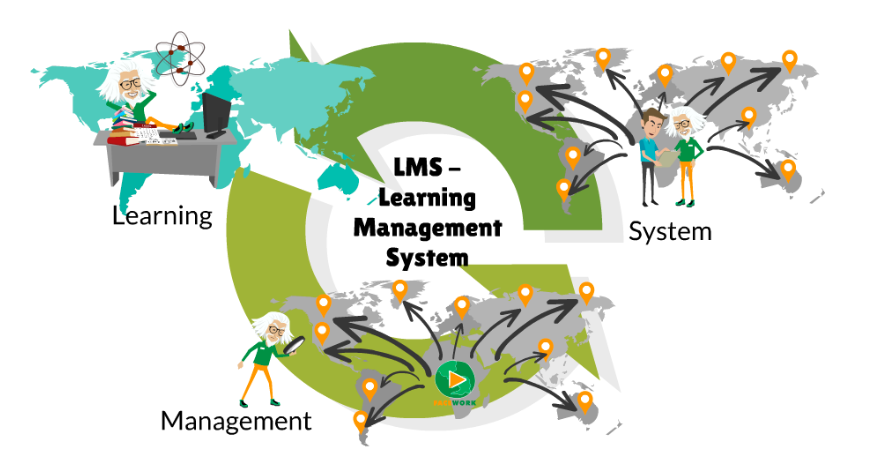
\includegraphics[scale=.5]{img/LMS}
		\end{center}
		\caption{Giới thiệu LMS}
		\label{refhinh1}
	\end{figure}
\end{center}
Learing Management System là tổ hợp gồm 3 từ riêng lẻ: Learning, Management và System. Ý nghĩa của 3 từ đó được giải thích như sau:
\begin{itemize}
	\item Ý nghĩa về Learning: Các chủ thể trong hệ thống học trực tuyến tạo ra các khóa học hay chương trình đào tạo, và muốn phân phối các sản giáo dục này đến những người sử dụng.
	\item Ý nghĩa về Management: Việc tạo ra các khóa học hay thay đổi, xóa bỏ là điều cần thiết. Bên cạnh đó, với Management, người dùng có thể sắp xếp, phân loại hay đánh giá các khóa học. Một cách đích thực, Management có nghĩa là sự quản lý các khóa học trực tuyến.
	\item Ý nghĩa về System: Như thông tin bên trên, LMS về cơ bản vẫn là một chương trình máy tính và là tập hợp của những công nghệ số, nên nhìn chung đây là một hệ thống, và người ta dùng hệ thống này để quản lý các khóa học/ chương trình đào tạo.
\end{itemize}
\subsection{Các thành tố cấu thành một LMS}
{Trên thế giới hiện tại có rất nhiều hệ thống LMS đến từ nhiều nhà cung cấp, nhưng cốt lõi, các hệ thống LMS này đều nhằm mục đích giải quyết các nhu cầu tương tác của các chủ thể chính trong hệ thống học trực tuyến, đó là người cung cấp nội dung học trực tuyến, người sử dụng nội dung học trực tuyến và người điều hành, quản lý tương tác học trực tuyến.}

{Theo cấu trúc, một LMS được cấu thành từ 2 thành phần chính:}
\begin{itemize}
	\item Thành phần công nghệ nền gồm các chức năng cốt lõi như tạo, quản lý và cung cấp các khóa học, chứng thực người dùng, cung cấp các dữ liệu hay thực hiện các thông báo,…Thành phần này được quản lý và điều khiển bởi người lập trình, người quản lý hệ thống.
	\item Thành phần thứ hai liên quan đến giao diện người dùng chạy trên nền các trình duyệt web (tương tự như Gmail/ Facebook). Thành phần này được dùng bởi các chủ thể trong hệ thống học trực tuyến như người quản lý, giảng viên và học viên.
\end{itemize}

{Theo chức năng, LMS là một tổ hợp gồm một số chức năng cốt lõi sau:}
\begin{itemize}
	\item Chức năng quản lý lưu trữ dữ liệu số: Chức năng này cho phép các chủ thể trên hệ thống E-Learning có thể đăng tải các khóa học cũng như các tài liệu số liên quan hỗ trợ người học. Các dữ liệu số được đăng tải có hệ thống phân loại theo định dạng tập tin, dung lượng, theo thời gian đăng tải,…và được kiểm soát nội dung.
	\item Chức năng bảo mật: Đây là chức năng rất quan trọng trong hệ thống LMS, nó bảo vệ hệ thống dữ liệu của các chủ thể một cách an toàn. Hơn thế nữa, các thông tin cá nhân liên quan các chủ thể hoặc các dữ liệu liên quan đến tài chính cũng được bảo vệ.
	\item Chức năng đáp ứng: 
	\begin{itemize}
		\item Tương thích đa chủng loại thiết bị truy cập: Chức năng này hỗ trợ nhiều thiết bị công nghệ truy cập hệ thống LMS như máy tính bàn, laptop, thiết bị di động, hay máy tính bảng,...
		\item Băng thông đảm bảo lưu lượng người dùng truy cập vào hệ thống học trực tuyến.
	\end{itemize}
	\item Chức năng đa chủ thể: Tính năng này hỗ trợ một lớp học/ một chương trình đào tạo trực tuyến có sự tham gia tương tác cùng lúc bởi nhiều giáo viên và nhiều học viên, họ đến từ nhiều nơi trên toàn thế giới.
	\item Chức năng đa ngôn ngữ: Một LMS dùng làm mục đích kinh doanh, vận hành trên môi trường Internet có thể tiếp cận một cá nhân bất kỳ tại một quốc gia nào đó trên thế giới. Cho nên, việc cho phép chuyển đổi các ngôn ngữ qua lại hoặc ít nhất là một ngôn ngữ quốc tế cần được tích hợp vào hệ thống LMS.
	\item Kiểm soát đăng ký: Khả năng kiểm soát và tùy chỉnh quá trình đăng ký học trực tuyến.
	\item Lịch: Chức năng này thiết lập lịch cho các chương trình học tập trực tuyến như lịch học, thời hạn khóa học, lịch thi,...
	\item Chức năng quản lý giao dịch: Chức năng này cho phép hệ thống LMS kiểm soát được các giao dịch phát sinh khi tương tác với các khóa học trực tuyến của các chủ thể: giao dịch giữa học viên với người cung cấp dịch vụ E-Learning (học phí); Giao dịch giữa người cung cấp dịch vụ E-Learning với tác giả khóa học (thù lao giảng viên/ tiền phân chia lợi nhuận khóa học) hay các giao dịch tiền ký gửi học theo hình thức ví điện tử,...
	\item Chức năng quản lý tương tác, hỗ trợ:
	\begin{itemize}
		\item Tương tác giữa các học viên: Chức năng này cho phép các học viên có thể trao đổi thông tin, trao đổi tài liệu qua hệ thống chat, email hoặc SMS,... nhằm tương tác hỗ trợ học tập.
		\item Tương tác giữa học viên với tác giả: Chức năng cho phép giữa học viên và tác giả khóa học/ chương trình đào tạo có thể trao đổi thông tin hoặc đánh giá, nhận xét lẫn nhau.
		\item Tương tác giữa học viên, giảng viên với quản trị hệ thống: Chức năng cho phép 2 chủ thể là người cung cấp kiến thức khóa học và người nhận khóa học tương tác trao đổi với quản trị hệ thống. Các vấn đề tương tác liên quan như các quy định, chế độ,...
	\end{itemize}
	\item Chức năng thi, kiểm tra: Chức năng này cho phép các học viên tham gia kiểm tra năng lực học tập hoặc xếp loại sau khai trải qua quá trình học. Các hình thức thi và kiểm tra phổ biến trên hệ thống LMS như trắc nghiệm, nhiệm vụ tương tác thông qua game,...
	\item Chức năng theo dõi, kiểm soát: Chức năng này cho phép người học hoặc chủ thể trung gian quản lý người học có thể kiểm soát tiến trình học tập cũng như năng lực người học qua từng giai đoạn.
\end{itemize}
\subsection{Ưu điểm của LMS}
Từ khi xuất hiện lần đầu được dùng để mô tả một phần hệ thống quản lý của hệ thống học tập PLATO K-12, LMS đã dần phát triển ngày càng đa dạng tương ứng với nhiều mô hình giáo dục khác nhau trên toàn thế giới. Cho dù phân hóa theo đặc thù của từng đơn vị áp dụng, song, hệ thống LMS nói chung vẫn luôn trên mình như là một bản chất các ưu điểm:
\begin{itemize}
	\item Dễ dàng thích nghi và tái sử dụng theo thời gian.
	\item Có nhiều sự lựa chọn cho từng đối tượng tạo lập ra các chương trình giảng dạy như phương thức học tập, phương thức thanh toán, các hình thức tương tác, kiểm tra đánh giá,...
	\item Có thể dễ dàng tiếp cận các sản phẩm giáo dục của bên thứ 3 qua đó làm giảm chi phí sản xuất cho doanh nghiệp.
	\item Các doanh nghiệp có thể tận dụng LMS như là một công cụ để nhân viên tự đánh giá, kiểm tra qua đó rèn luyện nâng cao năng lực chuyên môn. Và với LMS, doanh nghiệp vừa tiết kiệm chi phí đào tạo vừa nhận được nhiều hơn các giá trị đến từ nhân viên.
\end{itemize}

\section{Tại sao chọn Moodle?}
\subsection{Giới thiệu về Moodle \cite{aboutmoodle}}
{Moodle (viết tắt của Modular Object-Oriented Dynamic Learning Environment) được sáng lập năm 1999 bởi Martin Dougiamas với mục đích tạo ra những khóa học trực tuyến có sự tương tác cao. Tính mã mở cùng sự linh hoạt của Moodle giúp người phát triển có khả năng thêm vào các module cần thiết một cách dễ dàng. Đây là phần quan trọng của hệ thống E-learning trong hỗ trợ học trực tuyến. Moodle được đánh giá là một thiết kế hướng tới giáo dục, dành cho những người làm trong giáo dục. Với giao diện trực quan dễ sử dụng, giáo viên chỉ mất một thời gian ngắn để làm quen và có thể sử dụng thành thạo. Moodle phù hợp với nhiều cấp học và hình thức đào tạo: phổ thông, đại học, cao đẳng, không chính quy hay trong các tổ chức, công ty.}


{Thông qua số liệu tháng 1 năm 2019 \cite{moodlestats} ta có được kết quả sau:}
\begin{center}
	\begin{table}[!htp]
		\centering
		\begin{tabular}{|l|r|}
			\hline 
			Trang web đã đăng ký & 107,517 \\ 
			\hline 
			Quốc gia đã đăng ký & 228 \\ 
			\hline 
			Khóa học đã đăng ký & 18,357,666 \\ 
			\hline 
			Lượng người dùng & 150,625,167 \\ 
			\hline 
		\end{tabular} 
		\caption{Thống kê Moodle}
		\label{bang1}
	\end{table}
\end{center}
\begin{center}
	\begin{table}[!htp]
		\centering
		\begin{tabular}{|l|r|}
			\hline 
			{\bf Quốc gia} & {\bf Số lượng người dùng} \\ 
			\hline 
			Mỹ & 9,971 \\ 
			\hline 
			Tây Ban Nha & 8,470 \\ 
			\hline 
			Mê Hi Cô & 5,287 \\ 
			\hline 
			Bra-xin & 5,260 \\ 
			\hline 
			Đức & 3,563 \\ 
			\hline 
			Anh & 3,458 \\ 
			\hline 
			Nga & 2,949 \\ 
			\hline 
			Ý & 2,923 \\ 
			\hline 
			Colombia & 2,498 \\ 
			\hline 
			Pháp & 2,464 \\ 
			\hline 
		\end{tabular} 
		\caption{Top 10 quốc gia đăng ký Moodle}
		\label{bang3}
	\end{table}
\end{center}

Từ kết quả trên ta có thể thấy được mức độ thông dụng của Moodle trong việc tạo ra một hệ thống quản lý học tập trực tuyến.
\subsection{Các chức năng cơ bản của Moodle \cite{featuremoodle}}
\begin{itemize}
	\item {\bf Trò chuyện:} Mô-đun trò chuyện cho phép người dùng có thể trao đổi thông tin theo thời gian thực. Đây quả thực là một cách hiệu quả để chúng ta có thể chia sẻ những sự hiểu biết cũng như những ý kiến cá nhân về chủ đề đang được thảo luận. Bên cạnh đó, mô-đun trò chuyện cũng chứa thêm những tính năng để quản lý cuộc trò chuyện một cách chủ động hơn.
	\item {\bf Cơ sở dữ liệu:} Mô-đun cơ sở dữ liệu cho phép giảng viên và sinh viên có thể hiện thị và tìm kiếm các mục trong một chủ đề, các mục này có thể là hình ảnh, tập tin, đường dẫn,... Tính năng đặc biệt của mô-đun cơ sở dữ liệu đó là chúng ta có thể tự thiết lập cơ sở dữ liệu để quyết định số lượng mục tối thiểu, tối đa mà một người dùng được phép tương tác,...
	\item {\bf Diễn đàn:} Diễn đàn là nơi để giảng viên, sinh viên cùng nhau thảo luận về nội dung bài học. Bằng việc đăng ký tham gia một diễn đàn, người tham gia sẽ nhận được thông tin những bài đăng mới nhất thông qua email. Giảng viên có thể thêm tất cả mọi người vào diễn đàn của mình nếu họ muốn vì thế giảng viên có thể liên hệ được với tất cả sinh viên trong khóa học của mình. Tất cả các khóa học của Moodle đi kèm theo là một diễn đàn Tin tức không thể xóa, tuy nhiên người dùng vẫn có thể thêm một diễn đàn mới.
	\item {\bf Bảng câu hỏi:} Mô-đun bảng câu hỏi cho phép giảng viên tạo ra một bản khảo sát hoặc bản câu hỏi để sinh viên điền vào nhằm đánh giá sự hài lòng của bạn về khóa học. Đặc biệt mô-đun này có tính năng ẩn danh người tham gia điền khảo sát giúp cho sinh viên thoải mái nêu lên những suy nghĩ của mình.
	\item {\bf Lịch biểu:} Mô-đun này cho phép giảng viên tạo ra những lịch biểu và yêu cầu sinh viên đăng ký vào những thời gian phù hợp với mình. Điều này là rất cần thiết cho các cuộc họp giữa sinh viên và giáo viên.
	\item {\bf Bài giảng:} Cho phép giảng viên tạo ra lộ trình bài học thông qua tài liệu. Nó gồm nhiều phần, mỗi phần thường kết thúc bằng một câu hỏi và một số câu trả lời có thể có. Tùy vào sự lựa chọn của học viên, nếu đúng họ sẽ được chuyển sang phần kế tiếp, còn nếu sai họ sẽ được đưa trở lại trang trước. Đây là một công cụ hữu ích để sinh viên học tập, nghiên cứu.
	\item {\bf Bài tập:} Mô-đun này cho phép sinh viên nộp bài một cách trực tuyến, bài tải lên có thể ở bất kỳ loại tệp nào (Word, Powerpoint, Zip, Video,...). Giảng viên có thể chấm điểm dựa vào đó và đưa ra phản hồi.
	\item {\bf Bài kiểm tra:} Mô-đun bài kiểm tra cho phép giáo viên thiết kế các bài kiểm tra bao gồm nhiều câu hỏi. Đây là một công cụ rất tiện lợi cho các giảng viên. Thật vậy bài kiểm tra điện tử có thể làm nhiều việc mà bài kiểm tra truyền thống trên giấy không thể. Người dùng có thể tạo ra các loại câu hỏi khác nhau, mở ngẫu nhiên câu hỏi có trong ngân hàng câu hỏi, cho phép học viên làm lại câu hỏi nhiều lần và có tính năng chấm điểm ngay khi học viên kết thúc bài kiểm tra.
	\item {\bf Scorm:} Moodle có mô-đun cho cả hai định dạng là SCORM hoặc AICC cho phép bạn dễ dàng đóng gói, tái sử dụng nội dung đào tạo của mình hoặc từ một khóa học khác.
	\item {\bf Khảo sát:} Các cuộc khảo sát được tạo ra nhằm mục đích thu thập thông tin về mức độ hài lòng của người học đối với khóa học. 
	
\end{itemize}

\subsection{Nguyên nhân lựa chọn Moodle}
Tầm quan trọng của Moodle được thể hiện tốt trong nhiều báo cáo, được cộng đồng chấp nhận và có nhiều khóa học hiện nay trên hầu hết nhiều quốc gia đang hoạt động dựa trên nền tảng Moodle. Nó cung cấp cho người dùng nhiều tính năng hữu ích như đăng tin tức, bài tập, bài giảng, video,... Điểm mạnh nhất của Moodle là có một cộng đồng phát triển to lớn, các diễn đàn thảo luận về những tích cực, chia sẻ mẹo, mã nguồn giúp cho những người dùng mới dễ dàng tiếp cận hơn.

Để thấy rõ hơn vì sao chúng em lựa chọn Moodle để nghiên cứu và xây dựng công cụ hỗ trợ các khóa học trực tuyến. Theo tìm hiểu chúng em đưa ra những lý do sau: \cite{whymoodle}
\begin{itemize}
	\item Moodle là một OSS, nghĩa là người dùng có thể tải Moodle miễn phí, sử dụng và chỉnh sửa nó một cách cá nhân, thậm chí chúng ta cũng có thể phân phối nó theo các điều khoản của giấy phép GNU.
	\item Nó là một nơi để giáo viên có thể chia sẻ những tài liệu, giao bài tập, trao đổi,... với học viên của mình để việc học trở nên dễ dàng hơn.
	\item Moodle có thể sử dụng hầu hết các server viết bằng PHP, chúng ta có thể dễ dàng sử dụng và nâng cấp nó bằng ngôn ngữ PHP.
	\item Điểm đặc biệt của Moodle là sự kết hợp giữa việc dạy học với công nghệ, bên cạnh đó điểm mạnh của Moodle so với các hệ thống khác chính là nền tảng vững chắc của nó trong việc xây dựng một khóa học trực tuyến.
	\item Moodle được sử dụng trên nhiều quốc gia trên thế giới như số liệu bảng 2.1 chúng ta có thể thấy Moodle mạnh mẽ như thế nào.
	\item Moodle chạy được trên tất cả hệ điều hành thông dụng ngày nay như Windows, Linux, Unix. Nó được xây dựng bằng ngôn ngữ PHP, sử dụng MySQL, Oracle làm cơ sở dữ liệu.
	\item Moodle rất dễ dùng với giao diện trực quan, giáo viên chỉ cần một thời gian ngắn để làm quen và có thể sử dụng thành thạo Moodle. Do giao diện thiết kế sử dụng đơn giản nên giáo viên có thể tự cài và nâng cấp Moodle.
	\item Moodle thì rất tốt trong việc tạo điều kiện cho các sinh viên khoa học máy tính (công nghệ thông tin) có cơ hội để phát triển một module cho LMS Moodle. Sinh viên có thể xây dựng các module cho LMS Moodle và chia sẻ nó cho cộng đồng toàn cầu. 
	\item Tài liệu hỗ trợ của Moodle rất đồ sộ và chi tiết.
	\item Tuy là phần mềm mã nguồn mở, như chất lượng của Moodle rất tốt, chất lượng bằng hoặc tốt hơn Blackboard /WebCT trong nhiều khía cạnh. Bởi cộng đồng các nhà giáo dục, chuyên gia máy tính, và các chuyên gia thiết kế giảng dạy chính là những người phát triển Moodle, và kết quả là bạn có trong tay một sản phẩm đáp ứng tốt các yêu cầu người dùng.
	\item Bảng so sánh chức năng với các hệ thống khác cũng sẽ làm ta thấy rõ điều này (so sánh với các hệ thống thương mại (không phải mã nguồn mở) Blackboard và WebCT): \cite{moodle-blackboard-webct}
	\begin{center}
		\begin{table}[!htp]
			\centering
			\begin{tabular}{|c|c|c|c|}
				\hline 
				{\bf Tính năng} & {\bf Blackboard} & {\bf WebCT} & {\bf Moodle} \\ 
				\hline 
				Upload và chia sẻ tài liệu & Có & Có & Có \\ 
				\hline 
				Tạo một trang web và soạn thảo với HTML online & Không & Có & Có \\ 
				\hline 
				Thảo luận online & Có & Có & Có \\ 
				\hline 
				Đánh giá học viên & Không & Có & Có \\ 
				\hline 
				Chat Online & Có & Có & Có \\ 
				\hline 
				Xem các thông tin của học viên khác & Không & Không & Có \\ 
				\hline 
				Khảo sát và điều tra & Có & Có & Có \\ 
				\hline 
				Bảng xếp hạng & Có & Có & Có \\ 
				\hline 
				Học viên tự đánh giá bài làm của mình & Không & Không & Có \\ 
				\hline 
				Nhóm học viên & Có & Có & Có \\ 
				\hline 
				Nhật ký học viên & Không & Không & Có \\ 
				\hline 
				Đánh dấu thuật ngữ & Không & Không & Có \\ 
				\hline 
			\end{tabular} 
			\caption{Bảng so sánh Moodle, Blackboard và WebCT}
			\label{bang2}
		\end{table}
	\end{center}
	Thông qua bảng trên ta có thể thấy được tất cả các so sánh đều chỉ ra rằng Moodle là ưu việt nhất cho e-learning.
\end{itemize}

\subsection{Sự hạn chế của Moodle}
Bên cạnh những lợi ích mà Moodle mang lại thì chúng ta không thể không kể đến những mặt hạn chế của Moodle như sau:

\begin{itemize}
	\item Moodle thường chỉ dành cho lập trình viên. Nó trở nên rất phức tạp đối với người dùng bình thường. Thật vậy có hơn 66\% trong số người dùng là giáo viên, nhà nghiên cứu và quản trị viên. \cite{limitmoodle:1}
	\item Lập trình viên mới bắt đầu sẽ khó để cài đặt Moodle, vì có nhiều từ ngữ chuyên ngành kỹ thuật trong hướng dẫn cài đặt. \cite{limitmoodle:2}
	\item Moodle sẽ không hoạt động nếu như không có quản trị viên làm việc được với cả giáo viên và kỹ thuật viên để tạo ra tài nguyên trực tuyến. \cite{whymoodle}
	\item Mặc dù tài liệu tham khảo về Moodle rất nhiều nhưng hầu hết đều được viết bằng tiếng anh nên không phải ai cũng dễ dàng tiếp cận.
\end{itemize}

\section{Block(khối) trong Moodle}
\subsection{Khối là gì?}
Một khối thể hiện thông tin trong một khu vực nhỏ trong các cột bên. Trong ví dụ, khối hiển thị lịch, tin tức mới nhất hoặc là tên học viên đã ghi danh vào khóa học.

Block là các công cụ nằm ở cột bên trái và phải. Có nhiều Block được cung cấp sẵn cho bạn. Một số khối phổ biến là: People, Navigation, Settings, Search Forum, Campus Links and Calendar. Bạn có thể tạo một khóa học tùy ý bao gồm các khối liên quan đến khóa học của bạn. \cite{blockmoodle}

Các gói tiêu chuẩn có sẵn khi bạn cài đặt một Moodle. Bạn cũng có thể cài đặt thêm các khối có sẵn thông qua http://moodle.org/

Ở trang quản trị của Moodle, ta có thể thay đổi vị trí của các khối (khu vực quản trị, khu vực điều hướng, calendar…). Ta cũng có thể thêm các khối mới hoặc ẩn đi các khối đang hiển thị. Thậm chí ta có thể thiết lập các quyền cho các nhóm người dùng có thể thấy hoặc không thấy khối khi họ đăng nhập vào tài khoản của mình.

Tại khu vực quản trị, ta chọn Cài đặt trang ngoài \ Bật chế độ chỉnh sửa. Sau khi bật chế độ chỉnh sửa thì trên mỗi khối sẽ xuất hiện các button để cho ta thao tác.
\begin{center}
	\begin{figure}[htp]
		\begin{center}
			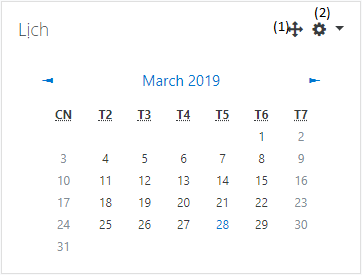
\includegraphics[scale=1]{img/lich}
		\end{center}
		\caption{Khối lịch trong Moodle}
		\label{refhinh2}
	\end{figure}
\end{center}
- Button (1) cho ta có thể dễ dàng kéo thả khối đến những vị trí khác trên giao diện.\\
- Button (2) cho phép ta thực hiện các thao tác như ẩn khối, xóa khối khỏi giao diện, thiết lập các nhóm người dùng có thể thấy hoặc không thấy khối.

Ta cũng có thể thêm một khối mới vào giao diện. Bằng cách lựa chọn khối mà ta muốn thêm trong mục "Thêm Khối".
\begin{center}
	\begin{figure}[htp]
		\begin{center}
			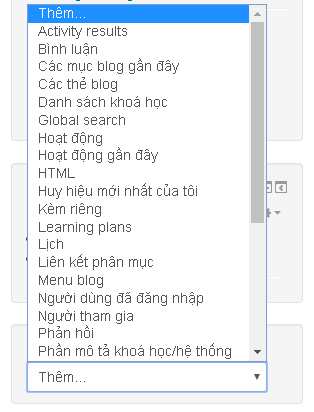
\includegraphics[scale=0.8]{img/addblock}
		\end{center}
		\caption{Giao diện lựa chọn block ta muốn thêm}
		\label{refhinh3}
	\end{figure}
\end{center}

\vskip 4cm
Giao diện sau khi thêm khối:
\begin{center}
	\begin{figure}[htp]
		\begin{center}
			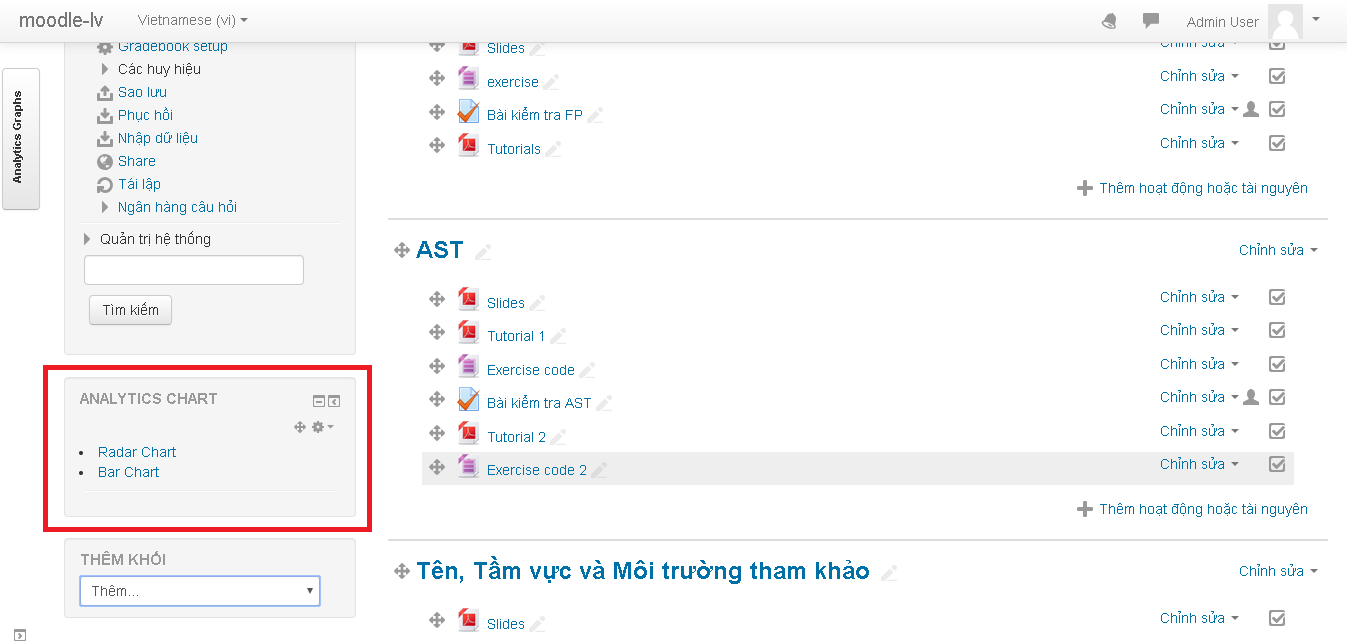
\includegraphics[scale=0.5]{img/block}
		\end{center}
		\caption{Khối đã được thêm vào}
		\label{refhinh4}
	\end{figure}
\end{center}

\subsection{Một số ví dụ về khối}
\subsubsection{Khối điều hướng:}
Khối điều hướng xuất hiện trong mỗi trang của trang web. Nó chưa một Menu cây mở rộng bao gồm: Trang chủ, các trang của hệ thống, hồ sơ và khóa học. Những gì xuất hiện trong khối điều hướng phụ thuộc vào vai trò của người dùng và họ đang ở đâu trong trang Moodle.
\begin{center}
	\begin{figure}[htp]
		\begin{center}
			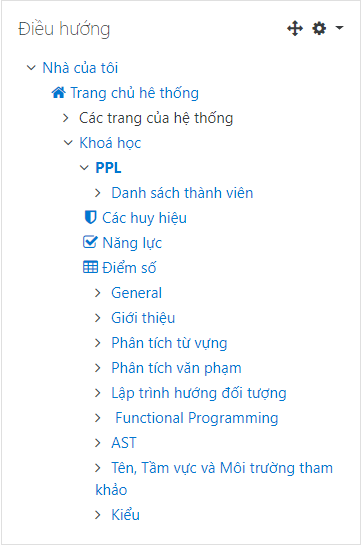
\includegraphics[scale=0.6]{img/khoidieuhuong}
		\end{center}
		\caption{Khối điều hướng}
		\label{refhinh5}
	\end{figure}
\end{center}

\subsubsection{Khối cài đặt:}
Khối cài đặt cung cấp các liên kết đến các trang cài đặt. Các mục Menu chính (Quản tri khóa học và hồ sơ của tôi) chứa nột Menu con và có thể được thu gọn hoặc mở rộng để hiển thị Menu như hình bên dưới.
\begin{center}
	\begin{figure}[htp]
		\begin{center}
			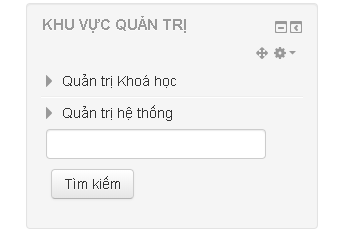
\includegraphics[scale=1]{img/khoicaidat}
		\end{center}
		\caption{Khối cài đặt}
		\label{refhinh6}
	\end{figure}
\end{center}

\subsubsection{Khối điều hướng bài kiểm tra:}
Khối điều hướng bài kiểm tra nằm ở góc trên bên phải. Bạn có thể sử dụng nó để di chuyển đến bất kì câu hỏi. Các hộp câu hỏi cho trang hiện tại được in đậm. Các câu hỏi được gắn cờ sẽ có “góc đỏ” trong hộp của câu hỏi.
\begin{center}
	\begin{figure}[htp]
		\begin{center}
			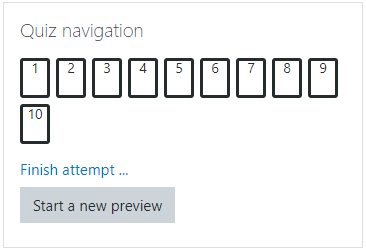
\includegraphics[scale=1]{img/khoibaikiemtra}
		\end{center}
		\caption{Khối điều hướng bài kiểm tra}
		\label{refhinh7}
	\end{figure}
\end{center}

\section{Tổng quan về ChartJS}
\subsection{ChartJS là gì? \cite{chartjs:1}}
ChartJS là một trong những dự án mã nguồn mở giúp cho mọi người có thể vẽ những biểu đồ thể hiện số liệu trên website một cách dễ dàng và đẹp nhất. Tính đến tháng 1 năm 2019 dự án này hiện có đến 41.000 stars và 2600 lượt commit trên Github và được cập nhật thường xuyên. Những ưu điểm nổi bật nhất của ChartJS là:
\begin{itemize}
	\item Dự án mã nguồn mở: cả cộng đồng phát triển và khắc phục lỗi.
	\item Tương thích tốt với HTML.
	\item Hơn 8 kiểu biểu đồ phổ biến nhất hiện nay.
	\item Có hỗ trợ responsive giúp hiển thị đẹp nhất trên tất cả các thiết bị từ Desktop, Tablet, Mobile.
\end{itemize}

\subsection{Cách cài đặt ChartJS \cite{chartjs:2}}
Có nhiều cách để cài đặt thư viện ChartJS nhưng chúng em xin đề cập những cách cài đặt phổ biến thông qua những công cụ sau:
\begin{itemize}
	\item npm: npm install chart.js --save
	\item Bower: bower install chart.js --save
	\item CDN: Truy cập link https://cdnjs.com/libraries/Chart.js
	\item Github: Truy cập link sau để tải về bản mới nhất https://github.com/chartjs/Chart.js/releases
\end{itemize}

\subsection{Sử dụng ChartJS trên web}
Để sử dụng ChartJS chúng ta cần thực hiện theo các bước sau: \cite{chartjs:3}
\begin{itemize}
	\item Khai báo thư viện ChartJS và Bootstrap.
	\item Tạo thẻ <canvas> trong trang web
	\begin{center}
		\begin{figure}[htp]
			\begin{center}
				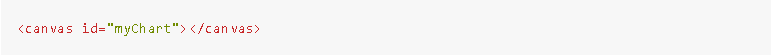
\includegraphics[scale=1]{img/canvas}
			\end{center}
			\caption{Thẻ canvas}
			\label{refhinh8}
		\end{figure}
	\end{center}
	\item Sử dụng Javascript để đăng ký biểu đồ.
	\begin{center}
		\begin{figure}[htp]
			\begin{center}
				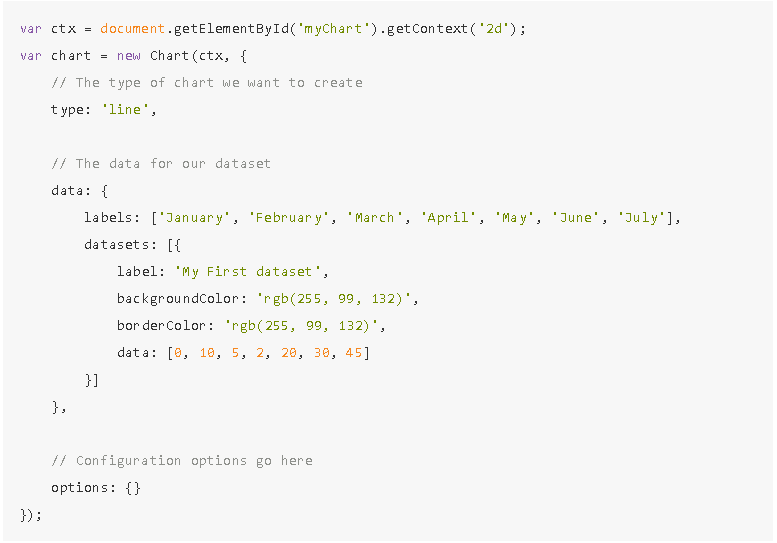
\includegraphics[scale=1]{img/chartjs}
			\end{center}
			\caption{Tạo một biểu đồ thông qua Javascript}
			\label{refhinh9}
		\end{figure}
	\end{center}
\end{itemize}